\documentclass[Measurement results]{subfiles}
\begin{document}
\newpage
\section{Measurement results}
\label{sec:Measurement results}

\subsection{Wordpress baseline performance measurement }
\subsubsection{Baseline measurement 1}
\label{sec:baseline_measurement_1}
\begin{verbatim}
~# httperf --server wp_without_naxsi.test.nl --uri /index.php \
--num-call 1 --rate 230 --num-conn 10000
httperf --client=0/1 --server=wp_without_naxsi.test.nl --port=80 \
--uri=/index.php --rate=230 --send-buffer=4096 --recv-buffer=16384 \
--num-conns=10000 --num-calls=1
Maximum connect burst length: 1

Total: connections 10000 requests 10000 replies 10000 test-duration 44.164 s

Connection rate: 226.4 conn/s (4.4 ms/conn, <=136 concurrent connections)
Connection time [ms]: min 0.7 avg 562.7 max 723.3 median 687.5 stddev 255.3
Connection time [ms]: connect 0.2
Connection length [replies/conn]: 1.000

Request rate: 226.4 req/s (4.4 ms/req)
Request size [B]: 86.0

Reply rate [replies/s]: min 203.2 avg 226.7 max 230.2 stddev 9.5 (8 samples)
Reply time [ms]: response 562.5 transfer 0.0
Reply size [B]: header 296.0 content 25.0 footer 1.0 (total 322.0)
Reply status: 1xx=0 2xx=0 3xx=8542 4xx=0 5xx=1458

CPU time [s]: user 1.30 system 42.87 (user 2.9% system 97.1% total 100.0%)
Net I/O: 90.3 KB/s (0.7*10^6 bps)

Errors: total 0 client-timo 0 socket-timo 0 connrefused 0 connreset 0
Errors: fd-unavail 0 addrunavail 0 ftab-full 0 other 0
\end{verbatim}

\subsubsection{Baseline measurement 2}
\label{sec:baseline_measurement_2}
\begin{verbatim}
# httperf --server wp_without_naxsi.test.nl --uri /index.php --num-call 1 \
--rate 190 --num-conn 10000
httperf --client=0/1 --server=wp_without_naxsi.test.nl --port=80 \
--uri=/index.php --rate=190 --send-buffer=4096 --recv-buffer=16384 \ 
--num-conns=10000 --num-calls=1
Maximum connect burst length: 1

Total: connections 10000 requests 10000 replies 10000 test-duration 52.656 s

Connection rate: 189.9 conn/s (5.3 ms/conn, <=10 concurrent connections)
Connection time [ms]: min 28.0 avg 31.8 max 51.9 median 31.5 stddev 2.0
Connection time [ms]: connect 0.2
Connection length [replies/conn]: 1.000

Request rate: 189.9 req/s (5.3 ms/req)
Request size [B]: 86.0

Reply rate [replies/s]: min 188.8 avg 189.9 max 190.2 stddev 0.4 (10 samples)
Reply time [ms]: response 31.6 transfer 0.0
Reply size [B]: header 321.0 content 0.0 footer 2.0 (total 323.0)
Reply status: 1xx=0 2xx=0 3xx=10000 4xx=0 5xx=0

CPU time [s]: user 8.93 system 43.73 (user 17.0% system 83.0% total 100.0%)
Net I/O: 75.5 KB/s (0.6*10^6 bps)

Errors: total 0 client-timo 0 socket-timo 0 connrefused 0 connreset 0
Errors: fd-unavail 0 addrunavail 0 ftab-full 0 other 0
\end{verbatim}

\subsection{Naxsi measurement 1}
\label{sec:Naxsi measurement 1}
\begin{lstlisting}[frame=single,caption=/etc/nginx/nbs.rules,backgroundcolor=\color{gray},breaklines=true,numbers=left,]
SecRulesEnabled;
DeniedUrl "/RequestDenied";

## check rules
CheckRule "$SQL >= 8" BLOCK;
CheckRule "$RFI >= 8" BLOCK;
CheckRule "$TRAVERSAL >= 4" BLOCK;
CheckRule "$EVADE >= 4" BLOCK;
CheckRule "$XSS >= 8" BLOCK;
\end{lstlisting}

\subsubsection{Resource usage}
\begin{figure}[H]
\centering
\caption{Wordpress baseline CPU usage}
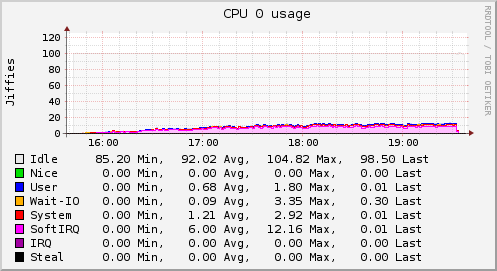
\includegraphics[scale=0.7]{images/results/baseline_wp/cpu.png}
\label{fig:Baseline Nginx CPU usage}
\end{figure}

\begin{figure}[H]
\centering
\caption{Wordpress baseline memory usage}
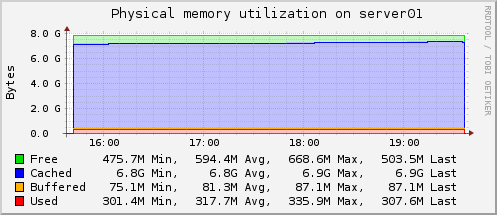
\includegraphics[scale=0.7]{images/results/baseline_wp/memory.png}
\label{fig:Baseline Nginx memory usage}
\end{figure}

\begin{figure}[H]
\centering
\caption{Wordpress baseline disk traffic}
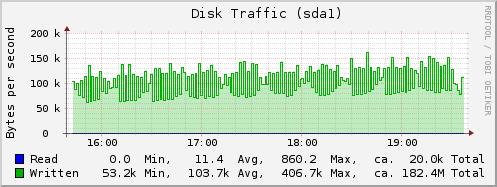
\includegraphics[scale=0.7]{images/results/baseline_wp/disk.png}
\label{fig:Baseline Nginx disk traffic}
\end{figure}

\begin{figure}[H]
\centering
\caption{Wordpress baseline interface traffic}
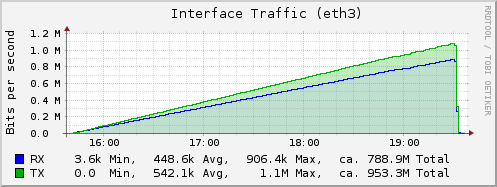
\includegraphics[scale=0.7]{images/results/baseline_wp/interface.png}
\label{fig:Baseline Nginx interface traffic}
\end{figure}

\subsection{HTTP 200 OK baseline performance measurement}

\subsubsection{Resource usage}
\begin{figure}[H]
\centering
\caption{HTTP 200 OK baseline CPU usage}
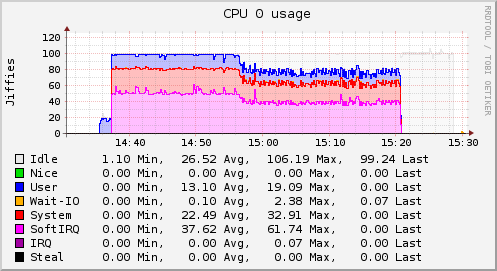
\includegraphics[scale=0.7]{images/results/baseline_200/cpu.png}
\label{fig:Baseline Nginx CPU usage}
\end{figure}

\begin{figure}[H]
\centering
\caption{HTTP 200 OK baseline memory usage}
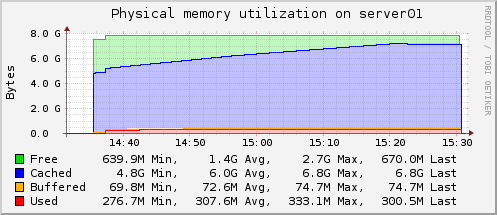
\includegraphics[scale=0.7]{images/results/baseline_200/memory.png}
\label{fig:Baseline Nginx memory usage}
\end{figure}

\begin{figure}[H]
\centering
\caption{HTTP 200 OK baseline disk traffic}
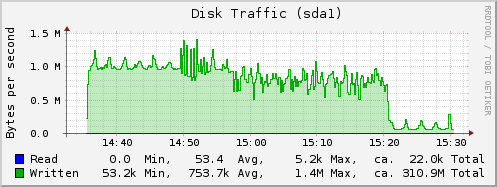
\includegraphics[scale=0.7]{images/results/baseline_200/disk.png}
\label{fig:Baseline Nginx disk traffic}
\end{figure}

\begin{figure}[H]
\centering
\caption{HTTP 200 OK baseline interface traffic}
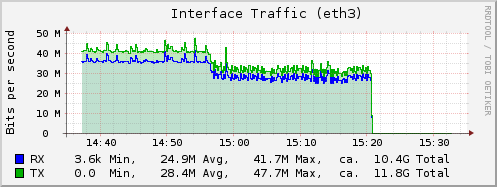
\includegraphics[scale=0.7]{images/results/baseline_200/interface.png}
\label{fig:Baseline Nginx interface traffic}
\end{figure}

% WORDPRESS with Naxsi
\subsection{Wordpress performance measurement with Naxsi}

\begin{lstlisting}[frame=single,caption=/etc/nginx/nbs.rules,backgroundcolor=\color{gray},breaklines=true,numbers=left,]
## check rules
CheckRule "$SQL >= 8" BLOCK;
CheckRule "$RFI >= 8" BLOCK;
CheckRule "$TRAVERSAL >= 4" BLOCK;
CheckRule "$EVADE >= 4" BLOCK;
CheckRule "$XSS >= 8" BLOCK;

# WordPress naxsi rules

### HEADERS
BasicRule wl:1000,1001,1005,1007,1010,1011,1013,1100,1200,
	1308,1309,1315 "mz:$HEADERS_VAR:cookie";
# xmlrpc
BasicRule wl:1402 "mz:$HEADERS_VAR:content-type";

### simple BODY (POST)
# comments
BasicRule wl:1000,1010,1011,1013,1015,1200 "mz:$BODY_VAR:post_title";
BasicRule wl:1000 "mz:$BODY_VAR:original_publish";
BasicRule wl:1000 "mz:$BODY_VAR:save";
BasicRule wl:1008,1010,1011,1013,1015 "mz:$BODY_VAR:sk2_my_js_payload";
BasicRule wl:1001,1009,1005,1016,1100,1310 "mz:$BODY_VAR:url";
BasicRule wl:1009,1100 "mz:$BODY_VAR:referredby";
BasicRule wl:1009,1100 "mz:$BODY_VAR:_wp_original_http_referer";
BasicRule wl:1000,1001,1005,1008,1007,1009,1010,1011,1013,1015,
   1016,1100,1200,1302,1303,1310,1311,1315,1400 
   "mz:$BODY_VAR:comment";
BasicRule wl:1100 "mz:$BODY_VAR:redirect_to";
BasicRule wl:1000,1009,1315 "mz:$BODY_VAR:_wp_http_referer";
BasicRule wl:1000 "mz:$BODY_VAR:action";
BasicRule wl:1001,1013 "mz:$BODY_VAR:blogname";
BasicRule wl:1015,1013 "mz:$BODY_VAR:blogdescription";
BasicRule wl:1015 "mz:$BODY_VAR:date_format_custom";
BasicRule wl:1015 "mz:$BODY_VAR:date_format";
BasicRule wl:1015 "mz:$BODY_VAR:tax_input%5bpost_tag%5d";
BasicRule wl:1100 "mz:$BODY_VAR:siteurl";
BasicRule wl:1100 "mz:$BODY_VAR:home";
BasicRule wl:1000,1015 "mz:$BODY_VAR:submit";
# news content matches pretty much everything
BasicRule wl:0 "mz:$BODY_VAR:content";
BasicRule wl:1000 "mz:$BODY_VAR:delete_option";
BasicRule wl:1000 "mz:$BODY_VAR:prowl-msg-message";
BasicRule wl:1100 "mz:$BODY_VAR:_url";
BasicRule wl:1001,1009 "mz:$BODY_VAR:c2c_text_replace%5btext_to_replace%5d";
BasicRule wl:1200 "mz:$BODY_VAR:ppn_post_note";
BasicRule wl:1100 "mz:$BODY_VAR:author";
BasicRule wl:1001,1015 "mz:$BODY_VAR:excerpt";
BasicRule wl:1015 "mz:$BODY_VAR:catslist";
BasicRule wl:1005,1008,1009,1010,1011,1015,1315 "mz:$BODY_VAR:cookie";
BasicRule wl:1101 "mz:$BODY_VAR:googleplus";
BasicRule wl:1007 "mz:$BODY_VAR:name";
BasicRule wl:1007 "mz:$BODY_VAR:action";
BasicRule wl:1100 "mz:$BODY_VAR:attachment%5burl%5d";
BasicRule wl:1100 "mz:$BODY_VAR:attachment_url";
BasicRule wl:1001,1009,1100,1302,1303,1310,1311 "mz:$BODY_VAR:html";
BasicRule wl:1015 "mz:$BODY_VAR:title";
BasicRule wl:1001,1009,1015 "mz:$BODY_VAR:recaptcha_challenge_field";

### BODY|NAME
BasicRule wl:1000 "mz:$BODY_VAR:delete_option|NAME";
BasicRule wl:1000 "mz:$BODY_VAR:from|NAME";

### Simple ARGS (GET)
# WP login screen
BasicRule wl:1100 "mz:$ARGS_VAR:redirect_to";
BasicRule wl:1000,1009 "mz:$ARGS_VAR:_wp_http_referer";
BasicRule wl:1000 "mz:$ARGS_VAR:wp_http_referer";
BasicRule wl:1000 "mz:$ARGS_VAR:action";
BasicRule wl:1000 "mz:$ARGS_VAR:action2";
# load and load[] GET variable
BasicRule wl:1000,1015 "mz:$ARGS_VAR:load";
BasicRule wl:1000,1015 "mz:$ARGS_VAR:load[]";
BasicRule wl:1015 "mz:$ARGS_VAR:q";
BasicRule wl:1000,1015 "mz:$ARGS_VAR:load%5b%5d";

### URL
BasicRule wl:1000 "mz:URL|$URL:/wp-admin/update-core.php";
BasicRule wl:1000 "mz:URL|$URL:/wp-admin/update.php";
# URL|BODY
BasicRule wl:1009,1100 "mz:$URL:/wp-admin/post.php|$BODY_VAR:_wp_http_referer";
BasicRule wl:1016 "mz:$URL:/wp-admin/post.php|$BODY_VAR:metakeyselect";
BasicRule wl:11 "mz:$URL:/xmlrpc.php|BODY";
BasicRule wl:11 "mz:$URL:/wp-cron.php|BODY";
BasicRule wl:2 "mz:$URL:/wp-admin/async-upload.php|BODY";
# URL|BODY|NAME
BasicRule wl:1100 "mz:$URL:/wp-admin/post.php|$BODY_VAR:_wp_original_http_referer|NAME";
BasicRule wl:1000 "mz:$URL:/wp-admin/post.php|$BODY_VAR:metakeyselect|NAME";
BasicRule wl:1000 "mz:$URL:/wp-admin/user-edit.php|$BODY_VAR:from|NAME";
BasicRule wl:1100 "mz:$URL:/wp-admin/admin-ajax.php|$BODY_VAR:attachment%5burl%5d|NAME";
BasicRule wl:1100 "mz:$URL:/wp-admin/post.php|$BODY_VAR:attachment_url|NAME";
BasicRule wl:1000 "mz:$URL:/wp-admin/plugins.php|$BODY_VAR:verify-delete|NAME";
BasicRule wl:1310,1311 "mz:$URL:/wp-admin/post.php|$BODY_VAR:post_category[]|NAME";
BasicRule wl:1311 "mz:$URL:/wp-admin/post.php|$BODY_VAR:post_category|NAME";
BasicRule wl:1310,1311 "mz:$URL:/wp-admin/post.php|$BODY_VAR:tax_input[post_tag]|NAME";
BasicRule wl:1310,1311 "mz:$URL:/wp-admin/post.php|$BODY_VAR:newtag[post_tag]|NAME";
# URL|ARGS|NAME
BasicRule wl:1310,1311 "mz:$URL:/wp-admin/load-scripts.php|$ARGS_VAR:load[]|NAME";
BasicRule wl:1000 "mz:$URL:/wp-admin/users.php|$ARGS_VAR:delete_count|NAME";
BasicRule wl:1000 "mz:$URL:/wp-admin/users.php|$ARGS_VAR:update|NAME";

# plain WP site
BasicRule wl:1000 "mz:URL|$URL:/wp-admin/update-core.php";
BasicRule wl:1000 "mz:URL|$URL:/wp-admin/update.php";
# URL|BODY
BasicRule wl:1009,1100 "mz:$URL:/wp-admin/post.php|$BODY_VAR:_wp_http_referer";
BasicRule wl:1016 "mz:$URL:/wp-admin/post.php|$BODY_VAR:metakeyselect";
BasicRule wl:11 "mz:$URL:/xmlrpc.php|BODY";
BasicRule wl:11 "mz:$URL:/wp-cron.php|BODY";
# URL|BODY|NAME
BasicRule wl:1100 "mz:$URL:/wp-admin/post.php|$BODY_VAR:_wp_original_http_referer|NAME";
BasicRule wl:1000 "mz:$URL:/wp-admin/post.php|$BODY_VAR:metakeyselect|NAME";
BasicRule wl:1000 "mz:$URL:/wp-admin/user-edit.php|$BODY_VAR:from|NAME";
BasicRule wl:1100 "mz:$URL:/wp-admin/admin-ajax.php|$BODY_VAR:attachment%5burl%5d|NAME";
# URL|ARGS|NAME
BasicRule wl:1310,1311 "mz:$URL:/wp-admin/load-scripts.php|$ARGS_VAR:load[]|NAME";
BasicRule wl:1000 "mz:$URL:/wp-admin/users.php|$ARGS_VAR:delete_count|NAME";
BasicRule wl:1000 "mz:$URL:/wp-admin/users.php|$ARGS_VAR:update|NAME";
\end{lstlisting}\footnote{\url{http://imil.net/wp/2012/12/30/wordpress-3-5-and-naxsi/}}

\begin{figure}[H]
\centering
\caption{HTTP 200 OK baseline CPU usage}
%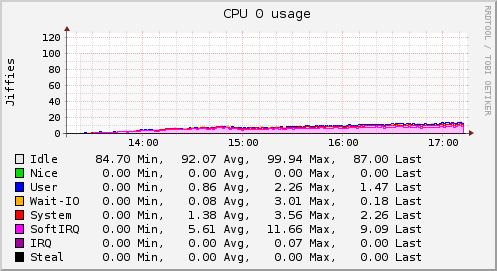
\includegraphics[scale=0.7]{images/results/wp_with_naxsi_1_to_230_concurrent_connections/cpu.png}
\label{fig:Baseline Nginx CPU usage}
\end{figure}

\begin{figure}[H]
\centering
\caption{HTTP 200 OK baseline memory usage}
%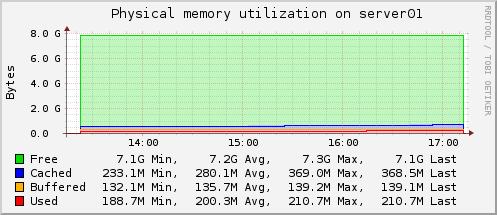
\includegraphics[scale=0.7]{images/results/wp_with_naxsi_1_to_230_concurrent_connections/memory.png}
\label{fig:Baseline Nginx memory usage}
\end{figure}

\begin{figure}[H]
\centering
\caption{HTTP 200 OK baseline disk traffic}
%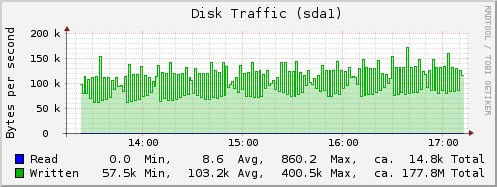
\includegraphics[scale=0.7]{images/results/wp_with_naxsi_1_to_230_concurrent_connections/disk.png}
\label{fig:Baseline Nginx disk traffic}
\end{figure}

\begin{figure}[H]
\centering
\caption{HTTP 200 OK baseline interface traffic}
%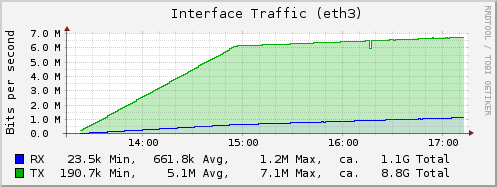
\includegraphics[scale=0.7]{images/results/wp_with_naxsi_1_to_230_concurrent_connections/interface.png}
\label{fig:Baseline Nginx interface traffic}
\end{figure}


\subsection{HTTP 200 OK performance measurement with Naxsi}
\subsubsection{Resource usage with allowed parameters}
\begin{figure}[H]
\centering
\caption{HTTP 200 OK baseline CPU usage}
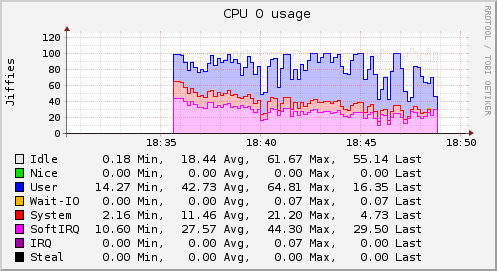
\includegraphics[scale=0.7]{images/results/200_with_naxsi_incremented_allowed_parameters/cpu.png}
\label{fig:Baseline Nginx CPU usage}
\end{figure}

\begin{figure}[H]
\centering
\caption{HTTP 200 OK baseline memory usage}
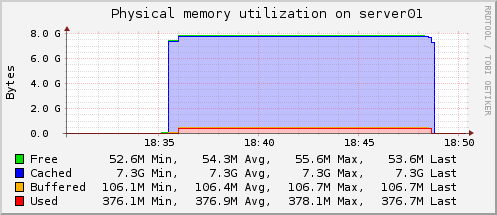
\includegraphics[scale=0.7]{images/results/200_with_naxsi_incremented_allowed_parameters/memory.png}
\label{fig:Baseline Nginx memory usage}
\end{figure}

\begin{figure}[H]
\centering
\caption{HTTP 200 OK baseline disk traffic}
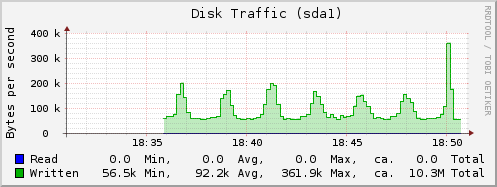
\includegraphics[scale=0.7]{images/results/200_with_naxsi_incremented_allowed_parameters/disk.png}
\label{fig:Baseline Nginx disk traffic}
\end{figure}

\begin{figure}[H]
\centering
\caption{HTTP 200 OK baseline interface traffic}
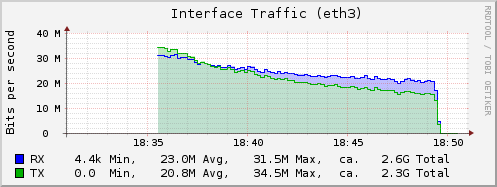
\includegraphics[scale=0.7]{images/results/200_with_naxsi_incremented_allowed_parameters/interface.png}
\label{fig:Baseline Nginx interface traffic}
\end{figure}

\subsubsection{Resource usage with disallowed parameters}
\begin{figure}[H]
\centering
\caption{HTTP 200 OK baseline CPU usage}
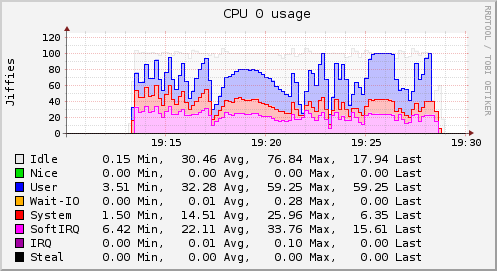
\includegraphics[scale=0.7]{images/results/200_with_naxsi_incremented_disallowed_parameters/cpu.png}
\label{fig:Baseline Nginx CPU usage}
\end{figure}

\begin{figure}[H]
\centering
\caption{HTTP 200 OK baseline memory usage}
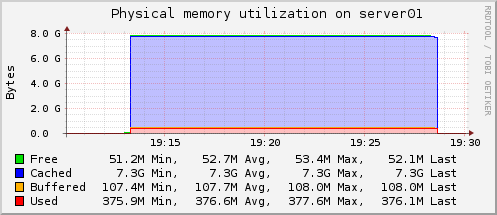
\includegraphics[scale=0.7]{images/results/200_with_naxsi_incremented_disallowed_parameters/memory.png}
\label{fig:Baseline Nginx memory usage}
\end{figure}

\begin{figure}[H]
\centering
\caption{HTTP 200 OK baseline disk traffic}
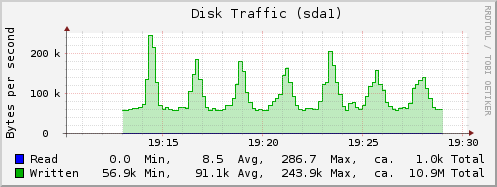
\includegraphics[scale=0.7]{images/results/200_with_naxsi_incremented_disallowed_parameters/disk.png}
\label{fig:Baseline Nginx disk traffic}
\end{figure}

\begin{figure}[H]
\centering
\caption{HTTP 200 OK baseline interface traffic}
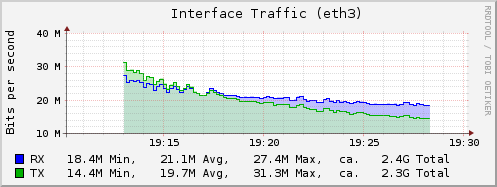
\includegraphics[scale=0.7]{images/results/200_with_naxsi_incremented_disallowed_parameters/interface.png}
\label{fig:Baseline Nginx interface traffic}
\end{figure}
\end{document}

